% Modules

\chapter{Modules} % Main chapter title

\label{Modules} % For referencing the chapter elsewhere, use \ref{Results} 

%----------------------------------------------------------------------------------------

% Define some commands to keep the formatting separated from the content 
\newcommand{\keyword}[1]{\textbf{#1}}
\newcommand{\tabhead}[1]{\textbf{#1}}
\newcommand{\code}[1]{\texttt{#1}}
\newcommand{\file}[1]{\texttt{\bfseries#1}}
\newcommand{\option}[1]{\texttt{\itshape#1}}

%----------------------------------------------------------------------------------------
\section{ITk Strip Module Design }
A ITK strip module\protect\footnote{For the scope of this thesis, while certain aspects of the barrel modules have been addressed, the primary emphasis will be directed toward the end-cap modules.} consists of $3$ main parts: sensor, hybrid, and power board.
The foundation of the ITk Strip module is made of a $300 \si{\micro\meter}$ thick silicon sensor. The hybrids including Kapton PCBs, read-out chips, and control chips, and a power control board which powers the whole module, are installed on the top of the sensor. Fig.\ref{fig:modulelayout} shows an illustrated view of the ATLAS ITk module, showcasing the silicon sensor, hybrid, and power boards, with their different components.\\

\begin{wrapfigure}{R}{7cm}
    \centering
    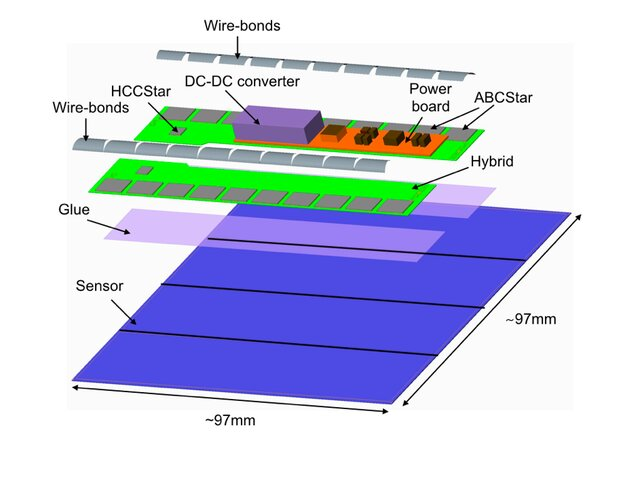
\includegraphics[width=7cm,height=10cm,keepaspectratio]{Figures/modules/modulelayout.jpg}
    \caption{An overview of an ITk module structure consisting of the silicon sensor, hybrid, and powerboard \cite{Collaboration:390920}.}
    \label{fig:modulelayout}
\end{wrapfigure}

\subsection{n$^+$-in-p silicon sensor}
The strip module is made of silicon, a semiconductor material that is sensitive to the presence of electric charge. The strip consists of a series of thin silicon strips arranged in a grid-like pattern. Each strip acts as an individual sensor capable of detecting the passage of charged particles and is made from silicon semiconductor material that has been doped with impurities to create specific types of charge carriers: p-type Silicon and n-type Silicon. In p-type material, atoms are doped with impurities that have one fewer electron in their outer shell than silicon. This creates "holes" or positively charged charge carriers where electrons are missing. On the other hand, in n-type material, atoms are doped with which have one extra electron in their outer shell compared to silicon. This results in an excess of negative charge carriers or free electrons.\\
When p-type and n-type silicon regions come into contact, a depletion region forms due to diffusion and electrostatic forces. In this area, free carriers (electrons in n-type and holes in p-type) combine, leaving behind charged ions. This causes a region with no charge carriers, making it insulating. A bias voltage is applied across the p-n junction, in a reverse bias configuration for silicon strip detectors. This reverse bias voltage widens the depletion region, improving the insulating properties. An illustration of a typical p-n junction is shown in Fig.\ref{fig:siliconpnjunction}.\\

\begin{figure}[h]
    \begin{subfigure}[b]{0.45\textwidth}
        \centering
        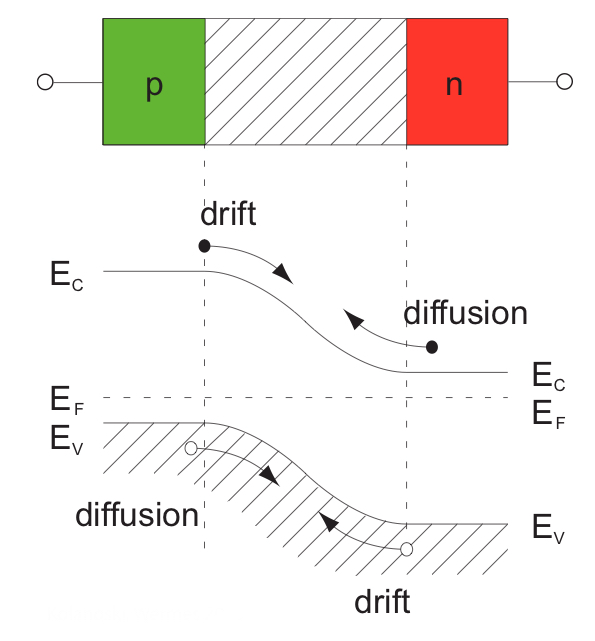
\includegraphics[width=6.5cm,height=10cm,keepaspectratio]{Figures/modules/Pnjunction.png}
        \caption{}\label{fig:siliconpnjunction}
    \end{subfigure}
    ~
    \begin{subfigure}[b]{0.45\textwidth}
        \centering
        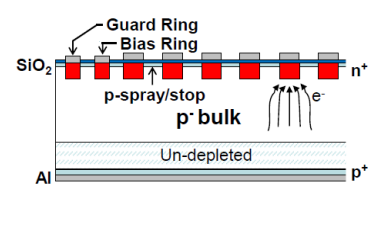
\includegraphics[width=6.5cm,height=10cm,keepaspectratio]{Figures/modules/striplayout.PNG}
        \caption{}\label{fig:striplayout}
    \end{subfigure}
    \caption{a) A schematic of a pn junction demonstrating the Fermi energy level ($E_f$), electron and hole movement, and the physical interaction within the semiconductor material\cite{kolanski}, and b) A schematic view of the n$^+$-in-p strip device\cite{striplayout}}
    
\end{figure}

When a charged particle passes through the silicon strip detector, it interacts with the silicon atoms, ionizing the particles interacting along its path. This ionization results in the creation of electron-hole pairs within the semiconductor material. The silicon strip detector is designed with a built-in electric field, which causes the newly created charges (electrons and holes) to move in opposite directions toward the positively and negatively biased electrodes, respectively. As the electrons and holes move toward the electrodes, they create an electric current in the silicon strips with a magnitude proportional to the energy deposited by the passing particle. The electric signals generated by the passage of particles through the silicon strips are amplified, digitized, and recorded by the detector's readout electronics. These signals are then analyzed by customized algorithms to reconstruct the trajectories of the charged particles and deduce their properties such as momentum, charge, and energy.\\

However, the biggest difference between the previous generation of the inner detector and the newly arrived ITk is the use of n$^+$-in-p strips. In this structure, the silicon bulk (the main body of the detector) is p-type. Near the surface of the silicon, there is a thin layer of heavily doped n-type material (n$^+$), which contains excess electrons as majority carriers. This creates a built-in electric field that facilitates the collection of charge carriers generated by particle interactions, which allows this configuration to acquire superior charge collection compared to the n-in-p configuration.\\

These strips can tolerate high levels of radiation and operate at voltages up to $700 \si{\volt}$. These properties give the advantage to the ITk module over the current ATLAS SCT modules to show exceptionally better signal performance after irradiation. n$^+$-in-p sensors deliver approximately twice as much charge compared to p-in-n sensors. Additionally, n$^+$-in-p technology is preferred due to lower costs, higher availability of foundries, and comparable signal sizes to n+-in-n sensors\cite{UNNO2013183}.\\

The silicon strip sensor as the sensing elements, which also are referred to as "Channels" when connected to the readout chips, are responsible for detecting and measuring the signals produced by charged particles. In ITK modules, channels are arranged in the form of very thin wafers of strips along the surface of the sensor. Each strip acts as an individual sensing element and is connected to readout electronics at one end. The number of channels in a strip sensor of ITk modules varies between each module due to the difference in geometry and the number of read-out chips.\\

%micrsocope picture

\subsection{Hybrid}
Hybrids act as a bridge between the readout electronics and the silicon sensor, enabling the conversion of sensor signals into digital data that can be handled and examined. These hybrids are designed to provide a platform for mounting and connecting the ABCStar readout chips, which are responsible for amplification, shaping, and digitizing the signals produced by particle interactions in the silicon sensor, and HCCstar which facilitates communication between the readout chips and the external control systems. \textcolor{blue}{By design, each hybrid is mounted on one side of the module, sitting directly on one of the sensors and bounded to both sensors separately. The part that the hybrid is mounted on is referred to as "Under", and the second part is referred to as "Away". The connection between the silicon stripes and the readout chips on the hybrids are made by $2$ thin wire threads, each connected to one side of the silicon strip (n and p)}  \\

%micrsocope picture

\subsection{Power board}
The front-end electronics of the hybrids get low voltage (LV) power from the power board via a DC-DC converter, which increases the voltage to the required levels. To ensure that the silicon sensor runs at the ideal voltage for signal detection, the power component also enables sensor high voltage (HV) biasing\cite{sykora2019itk} (high voltage creates an electric field within the sensor, which helps to accelerate and collect charge carriers (electrons and holes) generated by particle interactions). \cite{Collaboration:390920}. \\
In the heart of the power board, an Autonomous Monitoring And Control (AMAC) chip is installed in order to monitor and control the input and output electrical information of the module components. AMAC continuously monitors important parameters of the ITk module, such as voltage, and current, and if a parameter exceeds safe limits, it can take corrective actions. This might involve adjusting voltages or even shutting down the module to prevent damage.

\section{ITk Detector Design}
The new ATLAS ITk is an all-silicon detector, consisting of two major sub-systems of Pixel detector (ITk-Pixel) which will be placed closest to the beamline, and Strip detector (ITk-Strip) which would cover the bigger outer area. The strip detector itself, breaks down into two main subcategories of silicon strip modules, to cover the maximum area around the collision point: Barrel modules and End-cap modules.

\subsection{Barrel modules}
The beamline is encircled by four $2.8 \si{\meter}$-long cylinders, each consisting of $392$ staves consisting of $28$ modules on each (both sides, $14$ modules each), that make up the strip barrel. Two lengths of strips are used for the barrel: Long Strips (LS) with the length of $48.2  \si{\milli\meter}$ perform effectively in the lower occupancy zone at greater radii (layers L2 and L3), while Short Strips (SS) with the length of $24.1  \si{\milli\meter}$ are required for further subdivision at lower radii (layers L0 and L1). The main reason for this deviation in lengths is hidden in their final installation position around the beam. SS modules are located closer to the collision points and are expected to receive more flux from the collisions. To handle the higher flux of data, these modules have two dedicated hybrids with $10$ readout chips installed on each, which increases the processing power of each module consequently. On the other hand, LS modules are equipped with one hybrid and $10$ read-out chips and are located on the farther barrels from the beamline. 

\subsection{End-cap modules}
To give the best coverage, the strip end-caps (designated as end-cap A and end-cap C) feature six disks on each side.\\
 
The end-caps consist of $32$ identical "petals" on each disk. These petals are designed to cover the circular area of the barrel ends, and each hosts a total of $9$ modules with $6$ different geometries (R0 to R5). The sensors in the end-cap have two curving edges that form concentric arcs of circles centered at the disk's center (center of the beam), giving them an approximately trapezoidal shape. The difference in the geometry of the modules leads also to different strip lengths and different numbers of hybrids and read-out chips in each class. This difference is also important for the testing procedure because each module must be introduced separately due to its class to the testing environment to receive its own configuration for the test. 
Fig.\ref{fig:picModules} shows pictures of the LS and SS for the barrel, and R0 to R5 modules for the end-cap. (Higher resolution picture is shown in Fig.\ref{fig:picModules-large}). Also, Table.\ref{tab:moduleLaout} is listing the details of each module. 

\begin{figure}[h]
    \begin{subfigure}[b]{0.45\textwidth}
        \centering
        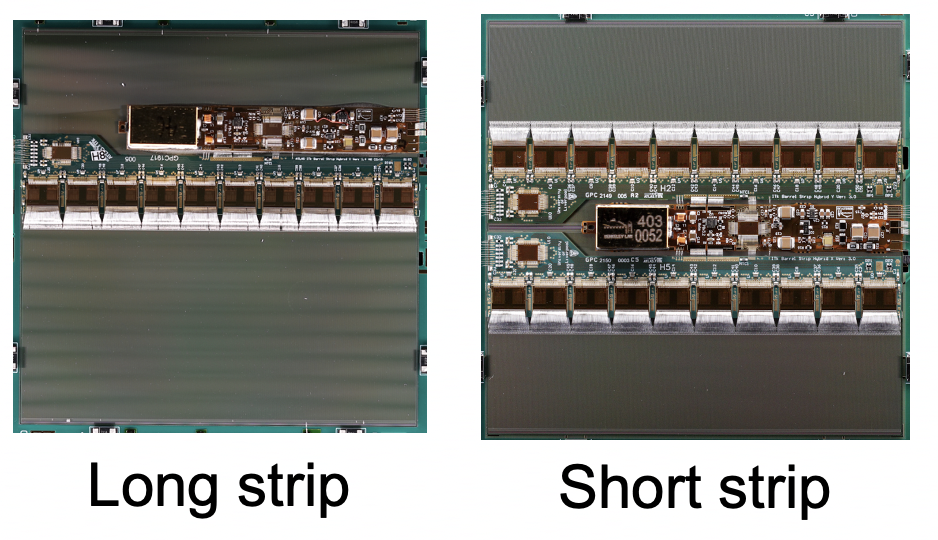
\includegraphics[width=7cm,height=15cm,keepaspectratio]{Figures/modules/Barrel_Modules.png}
        \caption{}\label{fig:barrel}
    \end{subfigure}
    \begin{subfigure}[b]{0.45\textwidth}
        \centering
        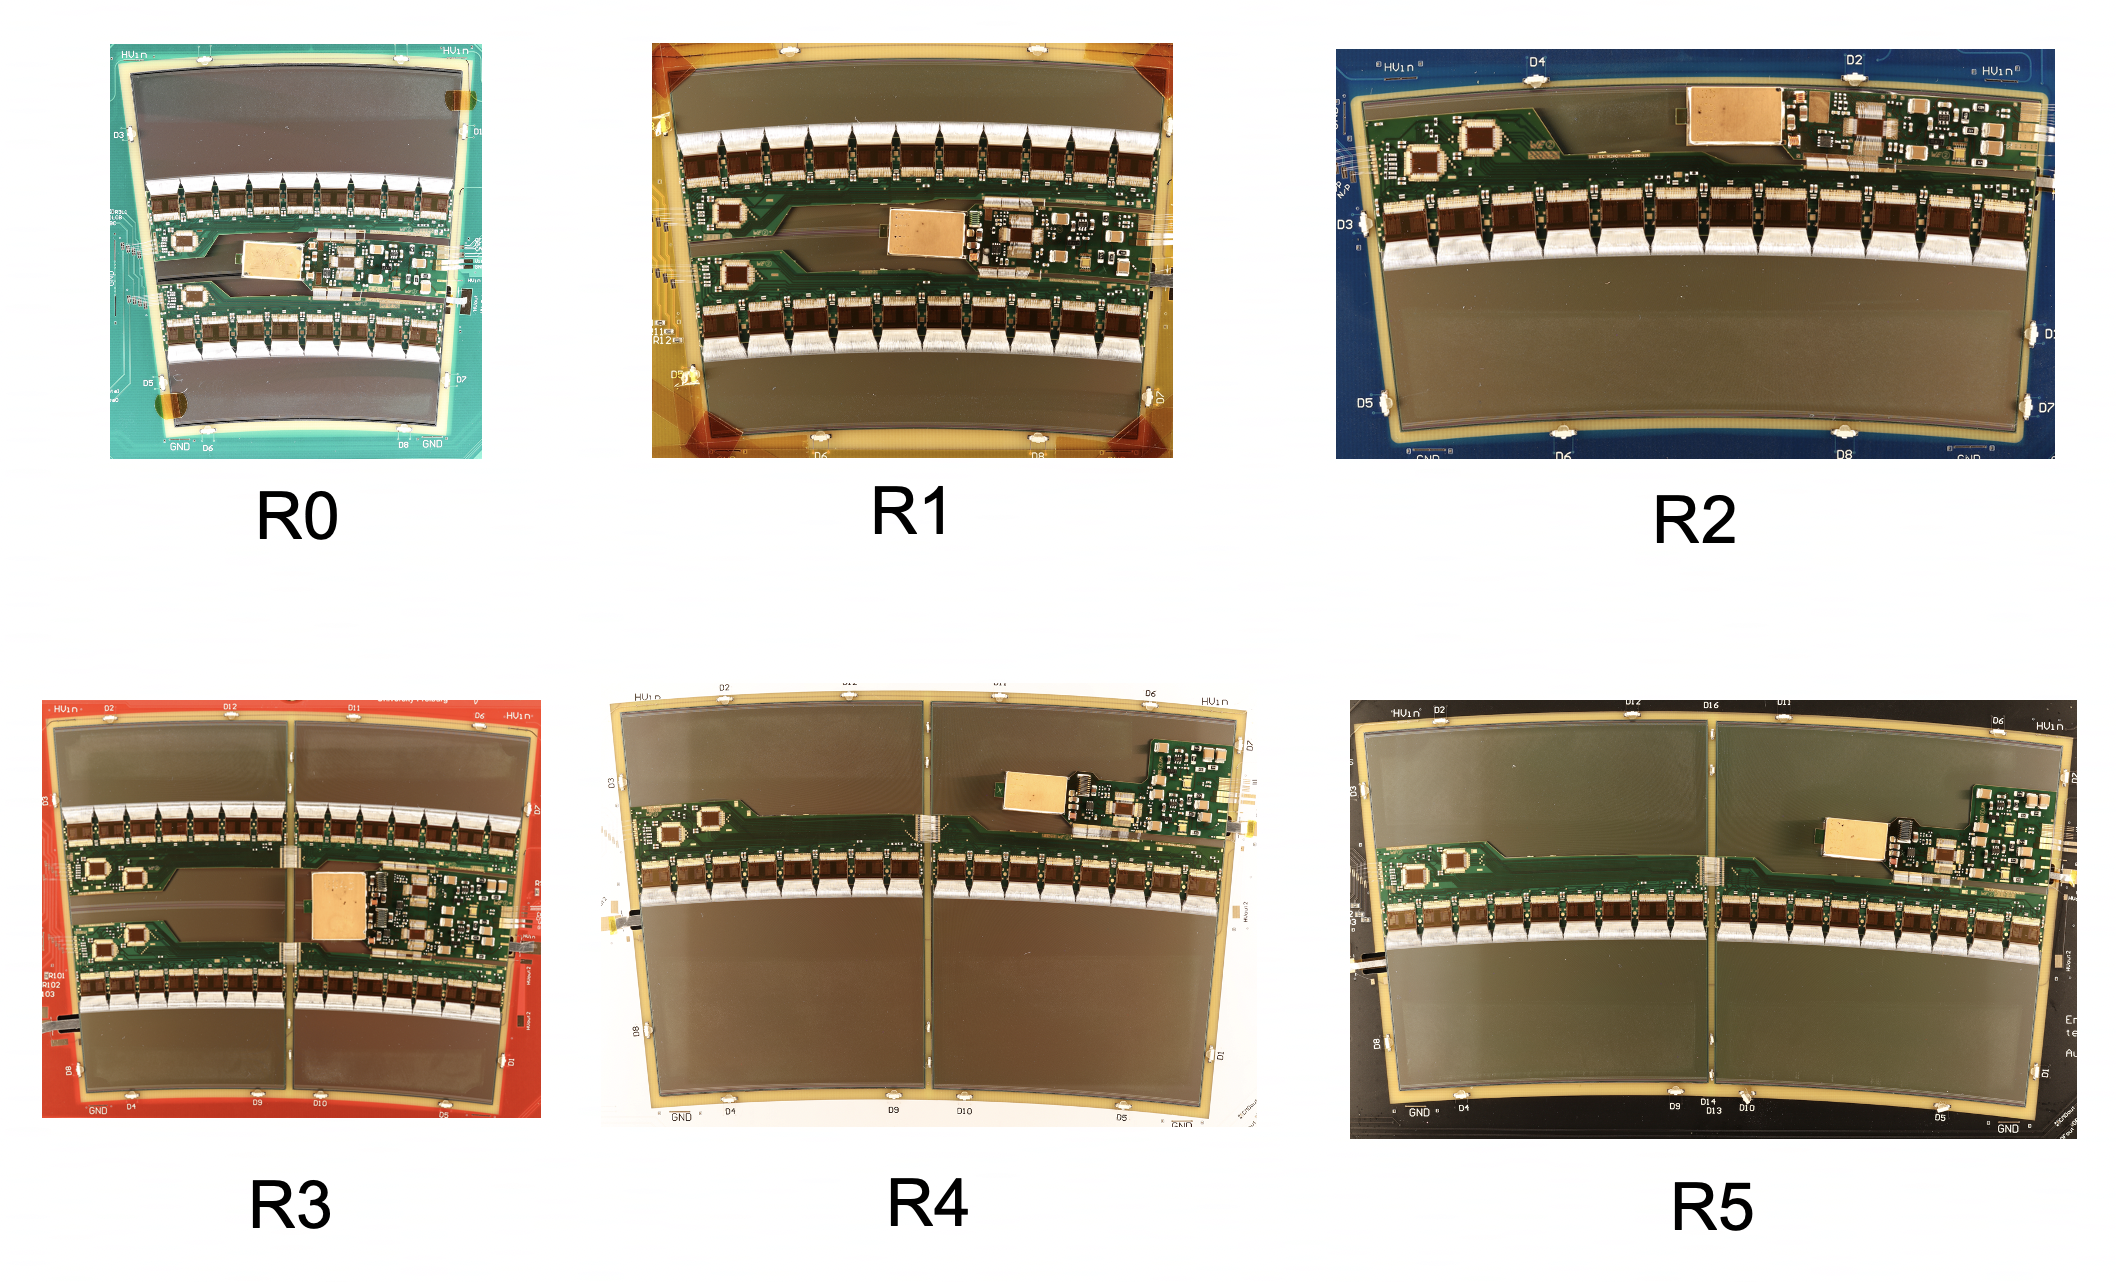
\includegraphics[width=7cm,height=15cm,keepaspectratio]{Figures/modules/EC_Modules.png}
        \caption{}\label{fig:endcap}
    \end{subfigure}
        \caption{Top view pictures of a) barrel modules including LS and SS, and b) end-cap modules including R0 to R5\cite{tishelman2024quality} }
        \label{fig:picModules}
\end{figure}

In total, an area of $165.25 \si{\meter\squared}$, ($104.86 \si{\meter\squared}$ for barrel area, $60.4 \si{\meter\squared}$ for end-caps), is covered by $17888$ modules in the new ITk detector. This area gives the coverage of $10^{\circ}$ of the beam axis, or $\pm 2.7$ units of pseudo rapidity to the strip system. Some additional overviews of the detector and modules' layout are shown in Fig.\ref{fig:additionalLayout}\cite{Collaboration:390920}. 


